\lecture\begin{lem} 
	Sei $ f: M \to N $ glatt ($M,N$ differenzierbare Mannigfaltigkeiten), sei $g$ eine Riemannsche Metrik auf $N$. Dann ist das Tensorfeld $ f^*g $ genau dann eine Metrik auf $M$, wenn $f$ eine \emph{glatte Immersion} ist, also $df$ überall injektiv ist.
\end{lem}

\begin{exmp*}
	$ f:(-\pi,\pi)\to \R^2,\ f(t) = (\sin(2t),\sin(t)) $\\
	\begin{minipage}{\linewidth}
		\begin{wrapfigure}{l}{0.1\textwidth}
			\wrapincfig{6_6}{0.1\textwidth}
		\end{wrapfigure}
		ist glatt und $ df(t) = (2\cos(2t),\cos(t)) $ hat Rang 1\\
		$\implies f^g$ ist eine Riemannsche Metrik, wenn $g$ eine Metrik auf $\R^2$ ist, z.B. mit der euklidischen Metrik $\bar{g}$:\\
		$\begin{aligned}
			f^*\bar{g} &= d(\sin(2t))^2 + d(\sin(t))^2\\
			&= (2\cos(2t)dt)^2 + (\cos(t)dt)^2\\
			&= (4(\cos(2t))^2 + (\cos(t))^2)dt^2
		\end{aligned}$
	\end{minipage}
\end{exmp*}

\begin{exmp*}
	Koordinatenwechsel:\\
	$ f(r,\theta) = \begin{pmatrix}
		r\cos(\theta)\\r\sin(\theta)
	\end{pmatrix} ,\ f: \R_{\geq 0} \times (0,2\pi) \to \R^2$\\
	$ \begin{aligned}
		f^*\bar{g} &= d(r\cos(\theta))^2 + d(r\sin(\theta))^2\\
		&= (\cos(\theta)dr - r\sin(\theta)d\theta)^2 + (\sin(\theta)dr + r\cos(\theta)d\theta)^2\\
		&= dr^2 + r^2d\theta^2
	\end{aligned} $
\end{exmp*}

\begin{defn*}
	Ist $ (M,g) $ eine Riemannsche Mannigfaltigkeit und $S \subset M$ eine Untermannigfaltigkeit, dann ist $\iota^*g$ eine Metrik auf $S$, wobei $\iota: S \hookrightarrow M$ eine Einbettung von $S$ in $M$ ist (Homöomorphismus auf $\iota(S)$, $\bound{d\iota}{p}$ injektiv $\foralll p$). Denn es ist
	\[ \iota \neq g_p(v,w) = g_p(d\iota(v),d\iota(w)) = g(v,w), \]
	wobei $v,w \in T_pS$ mit ihrer Einbettung in $T_pM$ identifiziert werden und $p \in S$ mit $p \in M$.
	\image{6_6 defn}{10cm}
\end{defn*}

\begin{exmp*}
	$ g_{\Sbb^2} := \iota^*\bar{g} $ auf $\Sbb^2$ \hfill (Standard-Metrik)\\
	In Koordinaten:
	\begin{align*}
		d\big(\cos&(\alpha) \sin(\beta)\big)^2 + d\big(\sin(\alpha)\sin(\beta)\big)^2 + d\big(\cos(\beta)\big)^2 \\
		=& \big(-\sin(\alpha)\sin(\beta)d\alpha + \cos(\alpha)\cos(\beta)d\beta\big)^2 \\
		&+ \big(\cos(\alpha)\sin(\beta)d\alpha + \sin(\alpha)\cos(\beta)d\beta\big)^2 + \big(-\sin(\beta)d\beta\big)^2\\
		=& \sin^2(\alpha) \sin^2(\beta) d\alpha^2 + \cos^2(\alpha) \cos^2(\beta) d\beta^2\\
		&+ \cos^2(\alpha) \sin^2(\beta) d\alpha^2 + \sin^2(\alpha) \cos^2(\beta) d\beta^2 + \sin^2(\beta) d\beta^2\\
		=& \sin^2(\beta) d\alpha^2 + d\beta^2
	\end{align*}
\end{exmp*}

\begin{exmp*}
	Sei $ H = \R_{\geq 0} \times \R,\ C \subset H $ eine 1-dimensionale Untermannigfaltigkeit und $ S_C $ die Rotationsfläche zu $C$,
	\[ S_C = \{(x,y,z) \mid \left( \sqrt{x^2+y^2},z \right) \in C \} \subset \R^2 \]
	\begin{minipage}{\linewidth}
		\begin{wrapfigure}{l}{6cm}
			%			\centering
			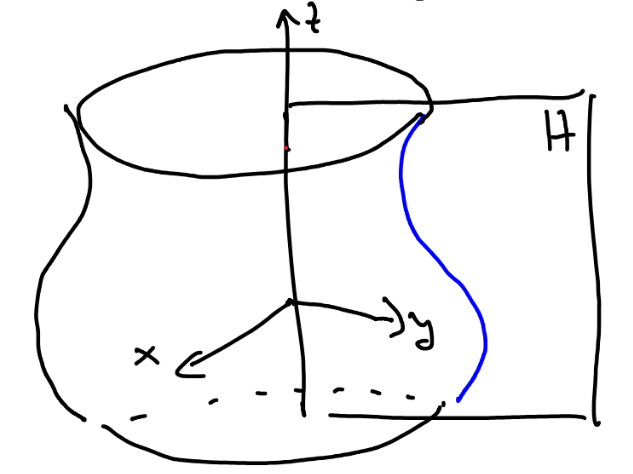
\includegraphics[width=6cm]{6_6 rot.png}
		\end{wrapfigure}
		Die von $\iota: S_C \hookrightarrow \R^3$ auf $S_C$ induzierte Metrik $\iota^*\bar{g}$ berechnet man lokal mit Parametrisierungen (wie oben):\\
		Sei $ \gamma(t) = (a(t),b(t)) $ eine lokale Parametrisierung von $C$. Dann ist
		\[ \varphi(t,\theta) = \big( a(t)\cos(\theta), a(t)\sin(\theta),b(t) \big) \]
		eine lokale Parametrisierung von $S_C$.
	\end{minipage}
	\begin{align*}
		\varphi^*\bar{g} &= d\big( a(t)\cos(\theta) \big)^2 + d\big( a(t)\sin(\theta) \big)^2 + d\big( b(t) \big)^2\\
		&= \big( \underbrace{a'(t)^2 + b'(t)^2}_{\|\gamma'(t)\|^2} \big)dt^2 + a(t)^2d\theta^2
	\end{align*}
\end{exmp*}

\subsection*{}

\begin{defn*}[(lokale) Isometrie]
	Sei $ f:M \to N $ glatt und $ (M,g_M),(N,g_N) $ Riemannsche Mannigfaltigkeiten. $f$ heißt \emph{Isometrie}, falls $f$ ein Diffeomorphismus ist und 
	$$f^*g_N = g_M.$$
	$f$ heißt \emph{lokale Isometrie}, falls $f$ ein lokaler Diffeomorphismus ist, der $ f^*g_N = g_M $ erfüllt.
\end{defn*}

\begin{rem}
	lokaler Diffeomorphismus: $ \foralll p \in M \ \existss U \subset M $ offen, $p \in U$, sodass $ \bound{f}{p} $ ein Diffeomorphismus auf $f(U)$ (offen in $N$) ist. Beachten Sie: $f$ ist genau dann ein lokaler Diffeomorphismus, wenn $ df_p: T_pM \to T_{f(p)}N $ ein Isomorphismus ist. (Das zeigt man in Koordinaten mit Hilfe des Satzes von der Umkehrfunktion auf Diff 2)
\end{rem}

\begin{exmp*}
	für einen lokalen, nicht globalen Diffeomorphismus
	\begin{itemize}
		\item $t \mapsto e^t, \R \to \R,$ ist nicht surjektiv.
		\item $ f: \R^2 \to \R^2, f(x,y) = (e^x\cos(y),e^x\sin(y)) $ ist nicht injektiv ($2\pi$-Periodizität)
	\end{itemize}
\end{exmp*}

\begin{defn*}
	Eine Metrik heißt \emph{flach}, falls sie lokal isometrisch zur euklidischen Metrik ist.
\end{defn*}

\begin{thm}\label{6.8}
	Sei $ (M,g) $ eine Riemannsche Mannigfaltigkeit. Dann sind äquivalent:
	\begin{enumerate}[label={\roman*})]
		\item $g$ ist flach
		\item $ \foralll p \in M \ \existss U \subset M $ offen, $p \in U, \varphi: U \to \R^n$ Karte, sodass in lokalen Koordinaten bezüglich $\varphi$ gilt:
			\[ g = \sum \delta_{ij} dx^i dx^j \]
	\end{enumerate}
\end{thm}

\begin{rem*}
	ACHTUNG: In Bemerkung \ref{6.1} hatten wir für ein fest gewähltes $p \in M$ eine Basis von $ T_pM $ gewählt, die $g_p$ in die Form $ \begin{pmatrix}
		1&&\\&\ddots&\\&&1
	\end{pmatrix} $ bringt. Die Aussage von \ref{6.8} ist stärker! Hier gibt es eine \emph{offene} Menge $ U \subset M $, auf der $g$ diese Form annimmt!
\end{rem*}

\begin{rem}
	$g$ flach $ \iff \foralll p \in M \ \existss U \subset M $ offen, $p \in U$ und ein kommutierendes orthonormales Vielbein\\
	kommutierend: $ \bound{(X_j \circ X_i - X_i \circ X_j)}{p} = 0 \qquad \foralll p \in U $
\end{rem}

\begin{lem}
	Sei $C$ eine zusammenhängende 1-dimensionale Untermannigfaltigkeit, eingebettet in $ H = \{r,z \mid r<0\} $. Sei $S_C$ die zugehörige Rotationsfläche. Dann ist $ \iota^*\bar{g} $ genau dann flach, wenn $C$ ein (offenes) Streckenstück ist.
\end{lem}

\subsection*{Riemannsche Mannigfaltigkeit $\to$ metrischer Raum:}

Für Kurven $ \gamma: I \to \R^n $ kennen wir schon die Länge 
\[ \int_I \|\gamma'(t)\|_E dt. \]
Analog betrachten wir nun zu einem stückweise glatten $ \gamma: [a,b] \to M $ ($(M,g)$ Riemannsche Mannigfaltigkeit)
\[ L_g(\gamma) = \int_a^b \|\gamma'(t)\|_g dt \quad \text{"Länge von $\gamma$"} \]
\[ \|\gamma'(t)\|_g = \sqrt{g_{\gamma(t)} (\gamma'(t), \gamma'(t))} \]

\begin{rem}
	\begin{enumerate}[label={\roman*})]
		\item $\gamma'$ ist außerhalb einer endlichen Menge von Punkten $\in [a,b]$ definiert und dort auch stetig und in anderen Punkten sind rechts- und linksseitige Grenzwerte definiert $\implies$ Integral ist wohldefiniert.
		\item Wie im Fall von Kurven im $\R^n$ zeigt man für ein stückweise glattes $\gamma: [a,b] \to M$:
		\[ L_g(\gamma) = L_g (\bound{\gamma}{[a,c]}) + L_g (\bound{\gamma}{[c,b]}) \]
		für $a \leq c \leq b$ und $L_g(\gamma)$ ist von der Parametrisierung unabhängig.
	\end{enumerate}
\end{rem}

\begin{lem}\label{6.12}
	Sei $ f: M \to N $ auf Riemannschen Mannigfaltigkeiten $(M,g_M)$ und $(N,g_N)$ eine lokale Isometrie. Dann ist $ L_{g_N}(f \circ \gamma) = L_{g_M} (\gamma) $ für die stückweise glatte Kurve $\gamma: [a,b] \to M$.
\end{lem}

\begin{defn*}[Riemannscher Abstand]\index{Riemannscher Abstand}
	Sei $ (M,g) $ eine zusammenhängende Riemannsche Mannigfaltigkeit und $ p,q \in M $. Dann nennt man
	\[ d_g(p,q) = \inf \{L_g(\gamma) \mid \gamma\ \text{stückweise glatte Kurve von $p$ nach $q$} \} \]
	den \emph{Riemannschen Abstand} von $p$ zu $q$.
\end{defn*}

\begin{rem*}
	Wir haben im Lemma gesehen, dass immer eine stückweise glatte Kurve existiert ($M$ zusammenhängend).
\end{rem*}

\begin{rem*}
	In $ (\R^n,\bar{g}) $ gilt: $ d_g(p,q) = \|p-q\|_E $ (kürzeste Verbindung: Streckenstück)
\end{rem*}